\chapter{Acoplamiento de modos $p_y$ y ángulo de invisibilidad}
En electroestática, es posible asociar las interacciones dipolares eléctricas con los polinomios de Legendre de orden 2, $P_2(\cos(\theta))=3\cos^2(\theta)-1$, con $\theta$ el ángulo que forman los dipolos entre sí. Se suele llamar \textit{ángulo mágico} al valor $\theta_m \approx 0.62$ rad, pues anula el término de interacción dipolar \citep{medmagic}. 

Este capítulo tiene como protagonistas a los llamados modos $p_y$ o modos dipolares verticales, cuya excitación es posible al superar la condición de corte (longitud de onda lo suficiemente pequeña y tanto contraste $\Delta n$ como ancho de la guía lo suficientemente grandes).



\section{Acopladores}
Al considerar qué sucede con el acoplamiento entre modos $p_y$ de guías elípticas, se pueden distinguir dos casos límite: 1) Para acopladores horizontales, el acoplamiento $C_\pi$ tiene signo positivo. 2) Para acopladores verticales, el acoplamiento $C_\sigma$ tiene signo negativo \cite{Pmodecoupling}. Esta fenomenología es análoga a la que sucede en los enlaces químicos $\sigma$ y $\pi$ de las cadenas de carbono orgánicas. Para comprobar este efecto, se fabricaron 20 dímeros con una distancia de separación de 25 $\mu$m y con una distancia de propagación de 15 mm y se varió el ángulo entre guías desde 0.00 rad hasta 1.57 rad. Utilizando el montaje SLM, se moduló un modo P: dos lóbulos del mismo tamaño con una diferencia de fase de $\pi$ entre ambos.


\begin{figure}[H]
	\centering
	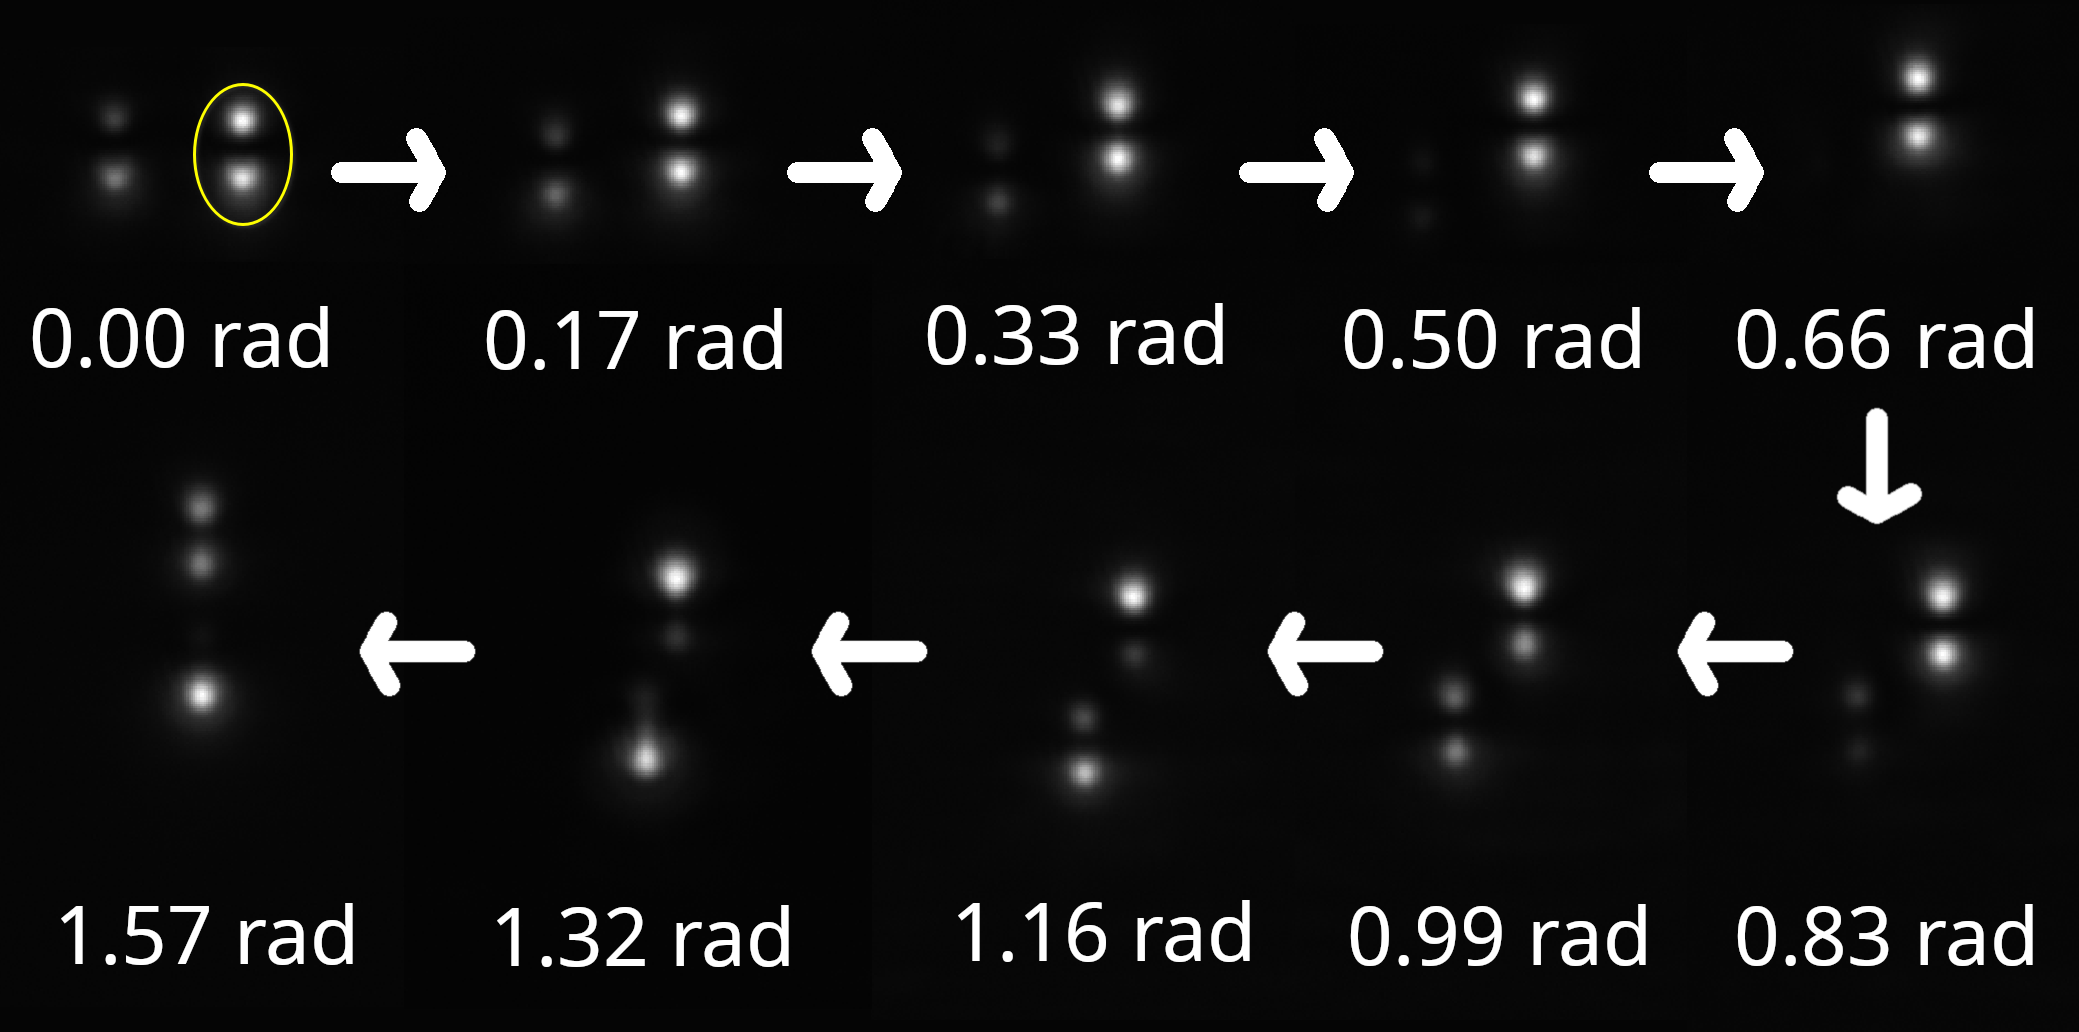
\includegraphics[trim={0 2cm 0 4cm},clip, width=\linewidth]{media/26um_15mm_angles_v2.png}
	\caption[Barrido de ángulo experimental.]{Barrido de ángulo experimental para una distancia de propagación de 15 mm. Se aprecia el efecto de ángulo mágico entre 0.50 y 0.66 rad. \label{fig:angulobarrido}}
\end{figure}
Se hizo un análisis de las imágenes como el descrito en la sección \ref{sec:analimag}. Luego, mediante la ecuación \ref{eqn:coupling-simp} para el acomplamiento dinámico, se caracterizó su comportameinto en función del ángulo $\theta$ medido desde la horizontal para una distancia de separación fija de 25 $\mu$m. El signo negativo se añadió de manera que la tendencia de los datos fuera continua, como se aprecia en la Figura \ref{fig:invisibility-coup}. 
\begin{figure}[H]
	\centering
	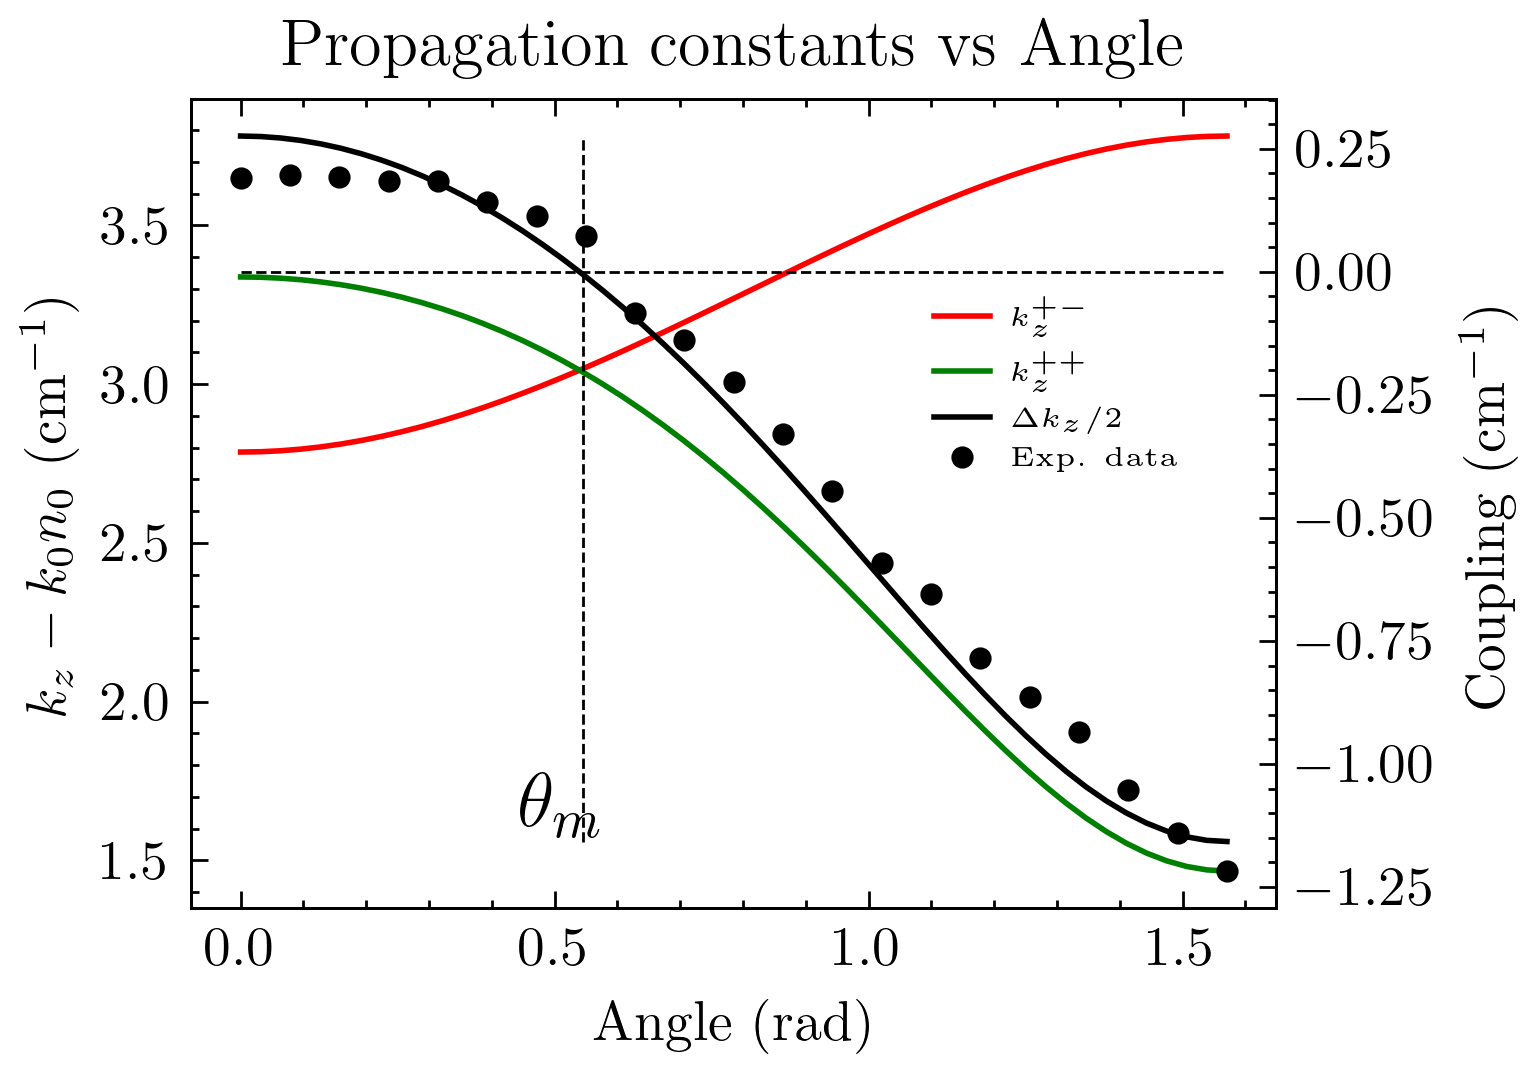
\includegraphics[width=0.8\linewidth]{codigo/eigenvalues_vs_angle.png}
	\caption[Constantes de propagación y acoplamientos en función del 
	ángulo para modos P.]{Constantes de propagación y acoplamientos en función del 
	ángulo para modos P, calculados numéricamente con EME. Se compara con los datos experimentales extraídos de la Figura \ref{fig:angulobarrido}. \label{fig:invisibility-coup}}
\end{figure}
\section{Redes tipo panal de abeja}
La red tipo panal de abeja es conocida por ser la red subyacente del grafeno. Su característica más relevante para efectos de esta tesis tiene relación con sus bandas de Bloch: ambas dispersivas y con la presencia de un punto de Dirac  \citep{honeycombdirac}.

Una vez encontrados los parámetros de fabricación de la sección anterior, se estudió el mismo efecto en una red tipo panal de abeja de forma que la distancia entre sitios permanece fija, sólo variando el ángulo (ver Figura \ref{fig:HCLBW}). 

\begin{figure}[H]
\centering
	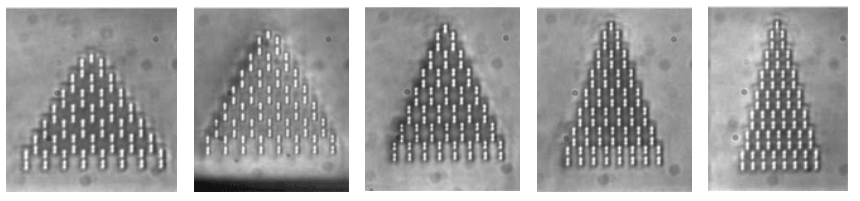
\includegraphics[width=0.8\linewidth]{media/honeycomb_lattices_bw.png}
	\caption[Imágenes microscópicas de redes fotónicas tipo panel de abeja de modos P.]{Imágenes microscópicas de redes fotónicas tipo panel de abeja de modos P iluminadas con luz blanca. \label{fig:HCLBW}}
\end{figure}

Un modelo a primeros vecinos consistiría en un acoplamiento vertical $\varkappa_\sigma$ y otro dependiente del ángulo $\varkappa_\theta$, sin embargo es necesario considerar acoplamientos hasta terceros vecinos y correcciones no ortogonales para describir adecuadamente la dinámica experimental.

\begin{figure}[H]
\centering
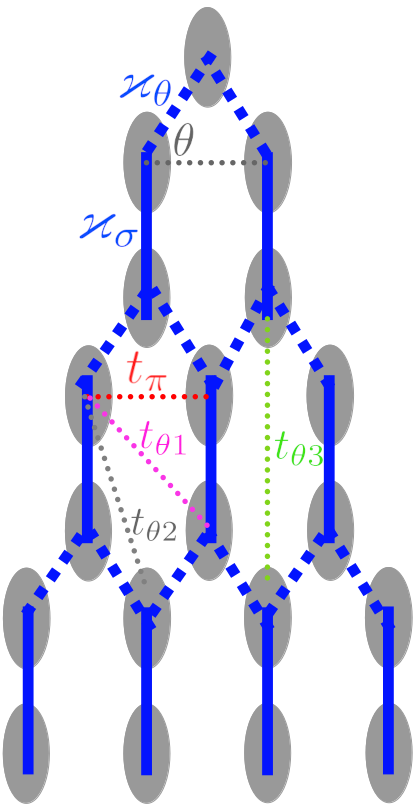
\includegraphics[width=0.3\linewidth]{media/honeycomb-lattice.png}
\caption{Esquema del modelo de honeycomb de modos P con terceros vecinos.}
\end{figure}